
% !TeX program = lualatex
%%

\documentclass[
	english,
	ruledheaders=section,%Ebene bis zu der die Überschriften mit Linien abgetrennt werden, vgl. DEMO-TUDaPub
	class=report,% Basisdokumentenklasse. Wählt die Korrespondierende KOMA-Script Klasse
	thesis={type=master},% Dokumententyp Thesis, für Dissertationen siehe die Demo-Datei DEMO-TUDaPhd
	accentcolor=1c,% Auswahl der Akzentfarbe
	custommargins=true,% Ränder werden mithilfe von typearea automatisch berechnet
	marginpar=false,% Kopfzeile und Fußzeile erstrecken sich nicht über die Randnotizspalte
	%BCOR=5mm,%Bindekorrektur, falls notwendig
	parskip=half-,%Absatzkennzeichnung durch Abstand vgl. KOMA-Script
	fontsize=11pt,%Basisschriftgröße laut Corporate Design ist mit 9pt häufig zu klein
%	logofile=example-image, %Falls die Logo Dateien nicht vorliegen
]{tudapub}


% Der folgende Block ist nur bei pdfTeX auf Versionen vor April 2018 notwendig
\usepackage{iftex}
\ifPDFTeX
	\usepackage[utf8]{inputenc}%kompatibilität mit TeX Versionen vor April 2018
\fi

%%%%%%%%%%%%%%%%%%%
%Sprachanpassung & Verbesserte Trennregeln
%%%%%%%%%%%%%%%%%%%
\usepackage[english, main=english]{babel}
\usepackage[autostyle]{csquotes}% Anführungszeichen vereinfacht

% Falls mit pdflatex kompiliert wird, wird microtype automatisch geladen, in diesem Fall muss diese Zeile entfernt werden, und falls weiter Optionen hinzugefügt werden sollen, muss dies über
% \PassOptionsToPackage{Optionen}{microtype}
% vor \documentclass hinzugefügt werden.
\usepackage{microtype}
\usepackage{todonotes}
%%%%%%%%%%%%%%%%%%%
%Literaturverzeichnis
%%%%%%%%%%%%%%%%%%%
\usepackage{biblatex}   % Literaturverzeichnis
\usepackage[utf8]{inputenc}
\usepackage[acronym]{glossaries}
\bibliography{DEMO-TUDaBibliography}


%%%%%%%%%%%%%%%%%%%
%Paketvorschläge Tabellen
%%%%%%%%%%%%%%%%%%%
%\usepackage{array}     % Basispaket für Tabellenkonfiguration, wird von den folgenden automatisch geladen
\usepackage{tabularx}   % Tabellen, die sich automatisch der Breite anpassen
%\usepackage{longtable} % Mehrseitige Tabellen
%\usepackage{xltabular} % Mehrseitige Tabellen mit anpassbarer Breite
\usepackage{booktabs}   % Verbesserte Möglichkeiten für Tabellenlayout über horizontale Linien

%%%%%%%%%%%%%%%%%%%
%Paketvorschläge Mathematik
%%%%%%%%%%%%%%%%%%%
\usepackage{mathtools} % erweiterte Fassung von amsmath
\usepackage{amssymb}   % erweiterter Zeichensatz
\usepackage{siunitx}   % Einheiten
\usepackage{amsmath}


\usepackage{xcolor}
\usepackage{listings}
\usepackage{xparse}


\usepackage{tikz}
\usepackage{geometry}
\usepackage[export]{adjustbox}



%Formatierungen für Beispiele in diesem Dokument. Im Allgemeinen nicht notwendig!
\let\file\texttt
\let\code\texttt
\let\tbs\textbackslash
\let\pck\textsf
\let\cls\textsf

\usepackage{pifont}% Zapf-Dingbats Symbole
\usepackage{layouts}
\newcommand*{\FeatureTrue}{\ding{52}}
\newcommand*{\FeatureFalse}{\ding{56}}




\begin{document}

\Metadata{
	title=Towards direct numerical simulations of mesopore imbibition, using a phase-field approach in OpenFOAM,
	author=Jan Kröger
}

\title{Towards direct numerical simulations of mesopore imbibition, using a phase-field approach in OpenFOAM}
%\subtitle{\LaTeX{} using TU Darmstadt's Corporate Design}
\author[J. Kröger]{Jan Kröger}%optionales Argument ist die Signatur,
\birthplace{Köln}%Geburtsort, bei Dissertationen zwingend notwendig
\reviewer{Professor Dieter Bothe \and Holger Marschall}%Gutachter

%Diese Felder werden untereinander auf der Titelseite platziert.
%\department ist eine notwendige Angabe, siehe auch dem Abschnitt `Abweichung von den Vorgaben für die Titelseite'
\department{math} % Das Kürzel wird automatisch ersetzt und als Studienfach gewählt, siehe Liste der Kürzel im Dokument.
\institute{Fachbereich Mathematik}
\group{Computational Multiphase Flow}

\submissiondate{\today}
\examdate{\today}

% Hinweis zur Lizenz:
% TUDa-CI verwendet momentan die Lizenz CC BY-NC-ND 2.0 DE als Voreinstellung.
% Die TU Darmstadt hat jedoch die Empfehlung von dieser auf die liberalere
% CC BY 4.0 geändert. Diese erlaubt eine Verwendung bearbeiteter Versionen und
% die kommerzielle Nutzung.
% TUDa-CI wird im nächsten größeren Release ebenfalls diese Anpassung vornehmen.
% Aus diesem Grund wird empfohlen die Lizenz manuell auszuwählen.
%\tuprints{urn=XXXXX,printid=XXXX,year=2022,license=cc-by-4.0}
% To see further information on the license option in English, remove the license= key and pay attention to the warning & help message.

% \dedication{Für alle, die \TeX{} nutzen.}

%%%%%%%%%%%%%%%%%\maketitle

\affidavit
% Es gibt mit Version 3.20 die Möglichkeit ein Bild als Signatur einzubinden.
% TUDa-CI kann nicht garantieren, dass dies zulässig ist oder eine eigenhändige Unterschrift ersetzt.
% Dies ist durch Studierende vor der Verwendung abzuklären.
% Die Verwendung funktioniert so:
%\affidavit[signature-image={\includegraphics[width=\width,height=1cm]{example-image}}, <hier können andere Optionen zusätzlich stehen>]

\tableofcontents
\listoftodos





\chapter{Introduction}
\label{chap: Introduction}
Many everyday phenomena that we observe are, contrary to expectations, not yet fully understood. This does not mean that they are not utilized in a variety of technical devices. In the case of wetting, we encounter many different things in everyday life, such as a drop on a window pane that seems to slide down randomly, or the sleeve of a sweater that seems to soak up water when washing hands.

Nature has a head start in this effect and has produced creatures that can walk on water because they take advantage of the water's surface tension. The flora also uses surface tension, whether it's trees that wouldn't reach the size we know without the capillary effect, or the lotus flower, which, with its water-repellent (hydrophobic) surface, ensures that water rolls off and takes dirt with it in the process.

Porous media, through their use in oxygenators, became lifesavers during the Corona pandemic by reoxygenating blood. The potential applications and necessities of this phenomenon could be demonstrated with many more examples. This work aims to describe the dynamics of capillary rise through simulations. A porous medium can be simplified as a collection of many small tubes. Insights from these small tubes can then be extrapolated to determine the behavior of the porous medium. Therefore, experiments with both porous media and individual capillaries are of great interest to understand how the rise in the capillary is designed. Simulations of these processes are also increasingly being carried out, as they have the advantage of fixing certain relevant material properties to examine their influence, or to look into areas that would not be possible with a conventional experimental setup.

In this work, the rise of a liquid column (water) in a capillary is investigated. Specifically, for a two-phase system, the area around the interface in the water phase is examined, and how dissipative processes in this region influence the rise of the water column. Possible phase changes (evaporation, boiling, condensation, etc.) are not taken into account. An isothermal and isobaric system is also assumed. All fluids treated are Newtonian, and the flow can be assumed to be Poiseuille flow. Furthermore, newly implemented boundary conditions of the used solver, which are supposed to better represent the behavior of the contact line and contact angle, will also be checked. 

This work will first discuss important findings in the description of capillary rise, the contact line, and the simulation of such problems with phase field methods in Chapter \ref{chap: BibliographyReview}. This is followed by an overview of the important influencing factors of wetting and their influence on the topics discussed in Chapter \ref{chap: wettingTheory}. Chapter \ref{chap: PhaseFieldMethod} provides an introduction to the phase field method and how it is implemented to simulate such problems. Chapter \ref{chap: Validation} shows that the solver used has already shown in many other simulations that it produces correct results and is applicable to these problems. Validation of the geometries used here is not possible due to their size, as they have a radius of 3 nm. It is not currently known that there are experiments that provide reliable results with a constant cross-section and such small radii. Subsequently, Chapter \ref{chap: CaseSetup} describes the setup of the simulations with descriptions of the geometry, material properties used, and solver settings. Finally, the results are discussed in Chapter \todo{ADD CHAPTER}, and an outlook for upcoming investigations is given in Chapter \todo{ADD CHAPTER}.

The solver used here is \texttt{phaseFieldFoam}, which is an extension of the open-source environment \texttt{OpenFOAM-extend}. The version used of \texttt{OpenFOAM-extend} is 5.0, and the version of the solver is still in development. The further development and maintenance of the solver are carried out through a cooperation between KIT (Karlsruhe Institute of Technology) and TU Darmstadt, especially by Dr.-Ing. Xuan Cai and Dr.-Ing. Holger Marschall. The simulations for this research were conducted on the Lichtenberg high-performance computer of the TU Darmstadt.




\todo[inline]{Here a introduction, but probably only after the most is done and the layout of the thesis is set.}

The dynamics of a rising fluid in the capillary is the subject of many processes. In nature, for example, trees would not be able to grow as high as they do without the capillary effect, and in technology many processes with a porous medium exist. Porous media can be simplified as many small tubes through which a fluid travels. Therefore, this process has long been of great interest in science and yet there are many uncertainties in the description of the dynamics.   

The Lucas Washburn equation, introduced in 1921 \cite{lucas_ueber_1918, washburn_dynamics_1921}, attempts to describe the height of the propagating fluid column as a function of time. This equation is sufficiently accurate for many applications.   
  
However, due to the assumptions made in the derivation of the equation, it is clear that it cannot be applied to every problem. Therefore, there are many approaches to adapt this equation to problems and simply maintain the behaviour of the equation. 

It is shown, that the Lucas Washburn equation has its problems in early stages of the imbibition\cite{bosanquet_lv_1923, quere_inertial_1997}\todo{check if quere1997 is also a source. Probably talked about that. Maybe even Washburn talked about that? }, due to the undefined behaviour for $t=0$ and neglecting the inertia of the fluid. 

The early stages of the imbibition process is yet to be understood and in this work we show how the different forces are acting on the meniscus for small time steps with a simulation of the such a problem. This simulations are done with the open source framework of foam extend, which is a fork of open foam. Here the department of mathmatics of the TU Darmstadt and the KIT developed a solver for a phase field approach. \todo{rework this regment.}

The developed solver phaseFieldFoam is maintained and developed by the department of MMA at the Tu darmstadt and ... KIT. It is using the Phase field approach to solve the Navier Stokes Equations (NSE).

In this work, first the attempts to describe the imbibition of a fluid in a capillay, especially for the early stages and small capillaies are discussed\todo{ref chapter}. Followed by the work, which has been done to simulate such problems with the phase field approach\todo{ref chapter}. Important interrelationships and derivations of the process of wetting is discussed, again followed by the equivalent numerical relations\todo{ref to both chapters}. How the simulations are setup and the results are in the chapers \todo{chapter} and \todo{chapter}.  


Lucas needed to prewet the tube to get the results he predicted 

In this work 

%\chapter{Bibliography Review}
%\label{chap: BibliographyReview}
%\input{bibliographyReview}

\chapter{Wetting Theory}
\label{chap: wettingTheory}
The wetting theory describes the interaction of fluids with solid surfaces. Many processes in nature, as well as in technology, are affected by this phenomenon. In this work, the focus is on the wetting properties in capillaries, which are often used as a simplification for understanding porous media or in other processes, such as the fact that trees would not be as tall as they are today without this effect. \todo{mention that we are considering spontaneous cap rise (no pressure or something like that)}

First, an overview of some types of wetting is presented \todo{ref}, and the concepts of contact angle and contact line are introduced. Subsequently, the surface tension \todo{ref} and its role in wetting are discussed. Since this work considers the dynamic rise of a water column in a capillary, the dynamic contact angle is also examined in Chapter \todo{ref chapter}, followed by a description of the capillary effect \todo{ref} and its significance for the rise of a fluid in a capillary. \todo{rework}

\section{Surface Tension}
\label{sec: Wetting_SurfaceTension}
Surface tension plays a significant role in the wetting of surfaces or in capillary rise. Therefore, it is essential to first clarify what surface tension is. In general, surface tension is a proportionality constant that depends on temperature, pressure, and the phases involved but is independent of the surface \cite{buttPhysicsChemistryInterfaces}. The interface separates the phases and can be interpreted differently. \todo{possibly ref to corresponding chapters here.}
On a molecular level, molecules attract each other (cohesion). The interaction between two phases is called adhesion. In the case of the interaction between a liquid and a solid, adhesion can usually be neglected. In Figure \ref{fig: WettingTheory_SurfaceTensionMolecules}, a water droplet surrounded by air is illustrated on the left. The black outer line thus represents the interface between the droplet and the air. If one now magnifies the transition area down to the molecular level (red area), one obtains the schematic representation on the right side. The blue circles are simplified representations of the water molecules, and the gray ones represent the surrounding air. Here, it is evident how, at the interface, the water molecules are no longer surrounded only by other water molecules, which is energetically unfavorable. However, since the system strives to transition into an energetically favorable state, it attempts to minimize the number of molecules lying at the interface \cite{buttPhysicsChemistryInterfaces}.

\begin{figure}[h]
    \centering
    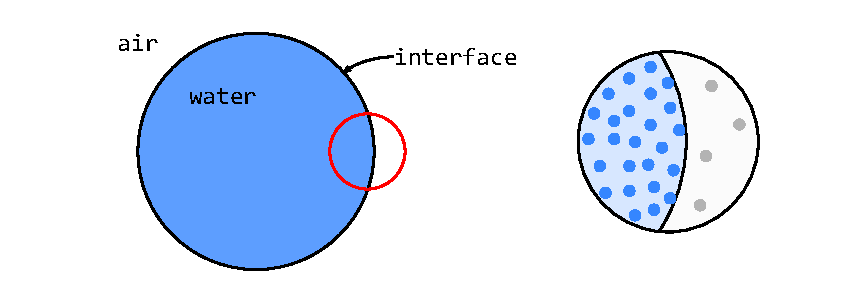
\includegraphics[width=.9\textwidth]{Pictures/moleculesAhesionCohesion_Wetting.pdf}
    \caption{Schematic of interacting molecules in a liquid droplet and its interaction with a vapor}
    \label{fig: WettingTheory_SurfaceTensionMolecules}
\end{figure}
To increase the surface area, molecules must be transported to the surface, and energy must be supplied to the system. Therefore, surface tension is also interpreted as the necessary energy required to carry a molecule to the surface.
\begin{equation}
    dE = \sigma \cdot dA
\end{equation}
with \(dE\) as the supplied energy and \(dA\) as the change in surface area.


\section{Wetting Phenomenon}
Despite the fact that the wetting of droplets is not considered in this work, it is appropriate to describe the fundamentals of wetting using this example. The concepts are the same, and many initial studies are based on this example.

In the case where the system is in equilibrium, Young \todo{ref} derived an equation relating surface tensions to the contact angle:
\begin{equation}
    \sigma_{LV} \cdot \cos\theta_e = \sigma_{SV}-\sigma_{SL}
    \label{eq: YoungsEQ}
\end{equation}
Where $\sigma_{LV}$ is the surface tension between the liquid and the gas, $\sigma_{SV}$ is from the solid to the gas, and $\sigma_{SL}$ is between the solid and the liquid (see Figure \ref{fig: YoungsLaw_ThreePhaseContactLine}).
\begin{figure}[h]
    \centering
    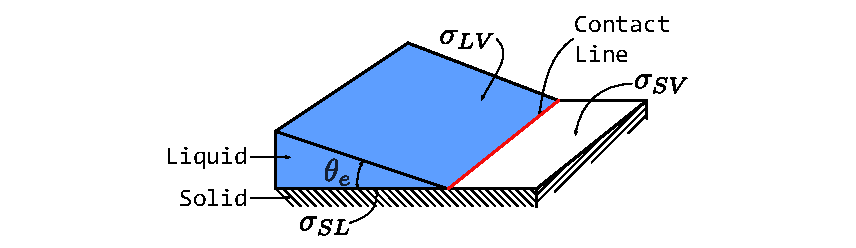
\includegraphics[width=.9\textwidth]{Pictures/YoungsLaw.pdf}
    \caption{Three Phase Contact Line}
    \label{fig: YoungsLaw_ThreePhaseContactLine}
\end{figure}
If $(\sigma_{SV}>\sigma_{SL})$ holds true, a contact angle less than $90°$ follows; otherwise, $90°\leq \theta_e<180°$. In the case where $\sigma_{SV}=\sigma_{SL}+\sigma_{LV}$, complete wetting of the surface occurs \cite{buttPhysicsChemistryInterfaces}.

When a droplet impacts a solid surface, different states can arise depending on the fluid-solid combination. At the point where the interface of the two fluids (droplet and surrounding fluid) meets the solid surface, the contact line is formed (see \ref{fig: YoungsLaw_ThreePhaseContactLine}; red line). Depending on the fluid-fluid-solid combination, a contact angle $\theta_e$ is established, where the suffix $e$ stands for equilibrium. In the case of complete wetting, the fluid spreads over the entire surface (see Figure \ref{fig: WettingTheory_WettingOfSurface} a)). This effect, however, is challenging to reproduce as it can be hindered by surface irregularities \todo{ref; i think it was butt}. As seen in Figure \ref{fig: WettingTheory_WettingOfSurface}(b-d)), states where a droplet forms on the surface are further subdivided. For a contact angle $\theta_e<90°$, it is termed hydrophilic (see \ref{fig: WettingTheory_WettingOfSurface}b)), for $\theta_e>90°$ it's hydrophobic (see \ref{fig: WettingTheory_WettingOfSurface}c)), and for a contact angle $\theta_e>120°$, it's superhydrophobic surfaces (see \ref{fig: WettingTheory_WettingOfSurface}d)). Developing superhydrophobic surfaces is also challenging.
\begin{figure}[h]
    \centering
    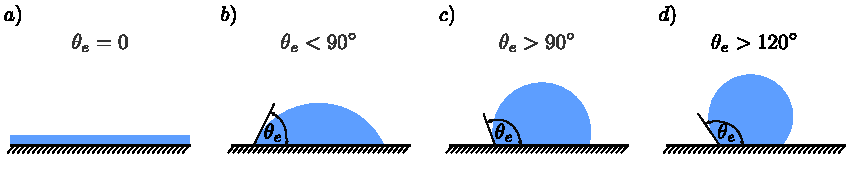
\includegraphics[width=.95\textwidth]{Pictures/DropletsAndWetting.pdf}
    \caption{Wetting of a surface}
    \label{fig: WettingTheory_WettingOfSurface}
\end{figure}
To curve the surface of the liquid, a pressure difference must exist. In the case of a sphere, Young and Laplace developed a relationship for the pressure difference in terms of the surface tension and radius as:
\begin{equation}
\label{eq: YoungLaplaceEQ}
    P_i - P_o = \Delta P =  \frac{2\sigma}{R}
\end{equation}
With $\Delta P$ being the pressure difference at the interface, $P_i$ as the pressure inside the droplet, $P_o$ the ambient pressure, and $R$ as the radius of the sphere. For a derivation, refer to \cite{buttPhysicsChemistryInterfaces}.


\subsection{Dynamic Weting}
Bisher wurden nur Zustände betrachtet, die Systeme im Gleichgewicht betrachten. Üblicherweise ist die Kontaktlinie jedoch in bewegung. Ist die Kontakilinie in Bewegung unterscheidet sich der Kontaktwinkel (dynamischer Kontaktwinkel $\theta_D$) von dem im Gleichgewichtszustand \cite{blake2006PhysicsMovingWetting}. Zur Bescheibung der Kontaktlinien dynamik wird der dynamische Kontaktwinkel, die relative geschwindigkeit der Kontatktlinie und der Gleichgewichtskontatktwinkel benötigt \cite{mohammadkarim2022ReviewPhysicsMoving, blake2006PhysicsMovingWetting, cox1986DynamicsSpreadingLiquids,huh1971HydrodynamicModelSteady,voinovHydrodynamicsWetting1977}.
Die beschreibung der Kontaktlinie ist jedoch aufgrund der tatsache schwierig, dass sich die Mikroskopische Ebene bis auf die makroskopische Ebene auswikt. 



In Abbildung \ref{fig: HDT_MKT_comp} sind verschiedene Ansichten auf die Kontatktlinie illustriert. Der rote Kreis in \textit{a)} weißt auf den betrachteten Bereich im rechts daneben stehenden bild hin und kann als eine Lupe verstanden werden. Vergrößern wir den Bereich in  \textit{a)} sieht man die interpretation der Kontatklinie aus sicht der Hydrodynamischen Theorie. Mit einem mikroskopischen Kontaktwinkel $\theta_m$ und dem dynamischen Kontaktwinkel $\theta_D$ (Abbildung \ref{fig: HDT_MKT_comp} \textit{b)}). Wird wieder auf die Kontatklinie fokussiert, sieht man die interpretation der molekular konetik Theorie (Abbildung \ref{fig: HDT_MKT_comp} \textit{c)}). Die illustrierten Punkte sollen auch hier wieder moleküle in vereinfachter Form darstellen. 



\begin{figure}[h]
    \centering
    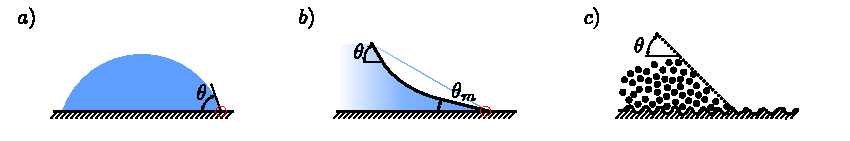
\includegraphics[width=.95\textwidth]{Pictures/ContactAngles_HDT_MKT.pdf}
    \caption{Hydrodynamic and Molecular Kinetic description of the Contact angle. Abbildung b) entsprocht dem Rot umkreisten Bereich in a), bzw. c) dem aus Bild b).}
    \label{fig: HDT_MKT_comp}
\end{figure}
\paragraph{Hydrodynamic Theory}
\label{paragraph: hydrodynTheory}
Der Hydrodynamische Ansatz löst die physik der Strömung mit Hilfe der Navier Stokes Gleichungen, bekommt jedoch bei angewandter Haftbedingung an der Kontaktlinie eine Singularität an der Kontaktlinie \cite{huh1971HydrodynamicModelSteady}. Um dieses Problem zum lösen wurde zum einen die Haftbedingung nahe der Wand gelockert oder die Lösung auf molekularer ebene beschnitten\cite{blake2006PhysicsMovingWetting}. In beiden Fällen wird eine kleine capillary number angenommen, was bedeutet, dass weit von der Kontaktlinie entfernt das Interface seine Gleichgewichtsform annimmt. 
Voinov \cite{voinovHydrodynamicsWetting1977} leitete dennoch eine Beschreibung der Kontaktlinie für einen sich ausbreitenden Tropfen in abhängigkeit der capillary number her. Eine generalisierte Variante von Cox \cite{cox1986DynamicsSpreadingLiquids} mit einigen korrekturtermen entwickelt\cite{carlsonCapillarityDynamicWetting2012,blake2006PhysicsMovingWetting}. So wird der dynamische Kontaktwinkel für $\theta_D \leq 3/4 \pi$ mit 
\begin{equation}
    \label{eq: Cox-Voinov}
    \theta_D^3-\theta_m^3= 9 Ca \ln\left(\frac{L}{L_m}\right) = 9 \frac{\mu u}{\sigma}\ln\left(\frac{L}{L_m}\right)
\end{equation}
Mit $L$ als makroskopische Weglänge und $L_m$ als mikroskopische Weglänge. Für die annahme, dass das Interface weit entfernd seine Gleichgewichtsform annimmt, wird $\theta_m = \theta_e$. Voinov selbst erkannte jedoch bereits an, dass auch $\theta_m$ anbängig von der Geschwindigkeit sein könnte\cite{voinovHydrodynamicsWetting1977,blake2006PhysicsMovingWetting}.\todo{cite lacis} 


\paragraph{Molekular Kinetic Theory}
Das Molekular Kinetik Modell beschreibt die Bewegung der Kontaktlinie mit einer statistischen Beschreibung der Molekularbewegung an der Kontaktlinie \cite{blake1969KineticsDisplacement}. 
Im gegensatz zum hydrodynamischen Modell beeinflussen die molekularen prozesse an der Kontatktlinie die der großen skalen. In dieser Betrachtung springen die Moleküle an der Kontaktlinie vor und zurück an adsorptionsstellen auf dem festen Untergrund. Die Geschwindigkeit der Kontaktlinie wird ermittelt, indem die differenz des vor und zurück springens multipliziert mit einer Sprungweite $\lambda$ multipliziert wird. Damit folgt die Beschreibung
\begin{equation}
    u=2\lambda\kappa_{0}\sinh\left(\frac{\sigma\left(\cos\theta_{e}-\cos\theta_{D}\right)}{2nk_{B}T}\right).
\end{equation}
Darin ist $n$ die Anzahl der adsorptionsstellen pro flächeneinheit, $k_0$ eine charakteristische Frequenz, $k_b$ die Boltzmann Konstante und $T$ die Temperatur.
Ist das system im Gleichgewicht, ist das vor und zurück springen im Gleichgewicht und die Kontatktlinie kommt zum stehen \cite{carlson2011DissipationRapidDynamic,blake2006PhysicsMovingWetting}. Ein Problem dieser Betrachtung ist es jedoch, dass dieses Modell eher qualitativ und rechenintensiv ist \cite{mohammadkarim2022ReviewPhysicsMoving}.







\subsection{Capillary Rise}
\label{sec: CapillaryRise}

Eine Kapillare ist ein sehr dünnes Rohr in denen durch Oberflächeneffekte eine Flüssigkeit ohne äußere Krafteinwirkung auf oder absteigt. In \ref{fig: classicCapillary} ist eine Kapillare mit bereits aufgestiegener Flüssigkeitssäule dargestellt. Darin sind ebenfall die bereits bekannten Oberflächenspannungen an ihren jeweiligen stellen markiert, sowie die wesentlichen Geometrischen parameter, wie Durchmesser ($2R$) oder höhe des entstandenen Meniskus $z$. Ebenfalls ist der resultierende Kontaktwinkel nach erreichen des Gleichgewichts gezeigt $\theta_e$. Das System in dieser Darstellung unterliegt auch Schwerkräften. 

\begin{figure}[h]
    \centering
    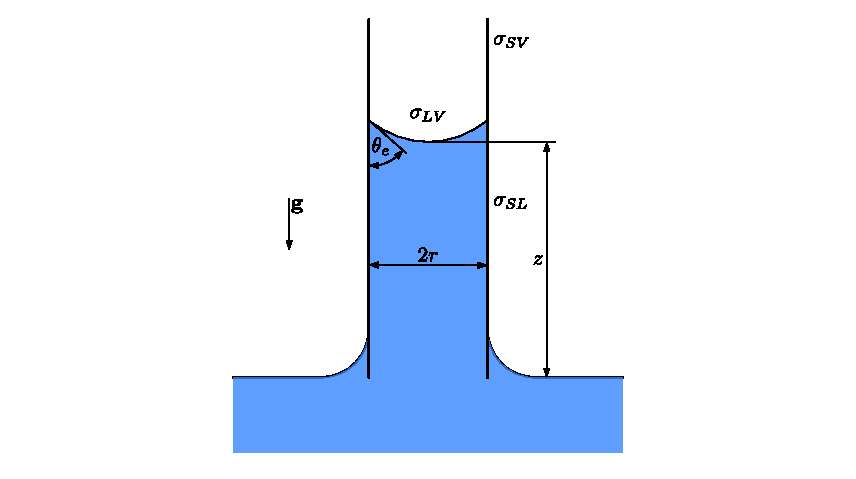
\includegraphics[width=.95\textwidth]{Pictures/classicCapillary.pdf}
    \caption{schematiche Darstellung einer Kapillare in einer Flüssigkeit nachdem diese in die Kapillare eingedrungen ist}
    \label{fig: classicCapillary}
\end{figure}
In dieser Arbeit wird ein solches System verwendet. Dabei gelten edoch weitere Bedingungen. Es wird angenommen, dass das System isobar, isotherm und die Flüssigkeit Newtonsch ist. Weiter gilt, dass während die Wassersäule in der Kapillare aufsteigt eine Poiseuille Strömung vorliegt und kein Phasenwechsel stattfindet. Weiter wird angenommen, dass die Viskosität der Gasphase vernachlässigbar ist. Mit diesen Annahmen und Randbedingungen kann die Newtondynamik in einer Kapillare als Gleichgewicht zwischen den Trägheitskräften zur Summe der Kapillaren Kräften, der Viskosen Kräfte und Hydrostatischen Kräfte \cite{fricke2023AnalyticalStudyCapillary}
\begin{equation}
\label{eq: NewtonBalanceForcesOnly}
    \frac{d}{dt}M(z,\dot{z}) = F_w - F_{\eta} - F_g
\end{equation}
Mit $M(z,\dot{z}) = \pi r^2 \rho z \dot{z}$ als das Moment, $F_g = \pi r^2 \rho g z$ als Gewichtskraft und $F_{\eta}$ als viskosen Widerstand, der sich aus der Annahme der mittleren Geschwindigkeit und vorliegenden Poiseuille Strömung zu $F_{\eta}=8\pi\eta z \dot{z}$ ergibt. Mit $\dot{z}$ als mittlere Geschwindigkeit. Die Kapillaren Kräfte folgen aus der vorherigen Beschreibung der Oberflächenspannung und der Änderung der Oberfläche des Meniskus bei änderung der aktuellen höhe zu:
\begin{equation}
    F_W=\sigma \frac{dA}{dz} = \sigma 2\pi r
\end{equation}
Die Oberflächenspannung $\sigma$ ist hierbei der zuwachs der Oberflächenenergie durch das Benetzen der festen Wand der Kapillare. Damit gilt $\sigma = \sigma_{SV}- \sigma_{SL}$. Diese Beschreibung ist bereits aus der Young Gleichung (\ref{eq: YoungsEQ}) bekannt. Damit folgt nach einsetzen für die Kapillaren Kräfte
\begin{equation}
    F_W = \sigma_{LV} \cdot \cos \theta_e 2\pi r.
\end{equation}
Damit folgt weiter für Gleichung \ref{eq: NewtonBalanceForcesOnly} nach einsetzen \cite{fricke2023AnalyticalStudyCapillary}
\begin{equation}
\label{eq: NewtonDynCapillary}
    \pi r^2 \rho \frac{d}{dt} (z \dot{z}) = \sigma_{LV} \cdot \cos \theta_e 2\pi r-8\pi\eta z \dot{z}-\pi r^2 \rho g z.
\end{equation}

Erste Beschreibungen von Bell und Cameron \cite{bell1906FlowLiquidsCapillary} haben die Aufstiegsdynamik nicht anhand von Gleichung \ref{eq: NewtonDynCapillary} beschrieben. Sie entwickelten anhand von Experimenten die Aufstiegsdynaik nach 
\begin{equation}
    z(t)^n = K\cdot t.
\end{equation}
Darin sind sowohl $n$ als auch $K$ von der Temperatur abhängige Konstanten. 1918 entwickelte Lucas \cite{lucas1918UeberZeitgesetzKapillaren} und 1921 Washburn \cite{washburn1921DynamicsCapillaryFlow} unter vernachlässigung der Trägheits- und Gravitationsterme die Lucas Washburn Gleichung wie folgt:
\begin{equation}
\label{eq: LW-Eq}
    z(t) = \sqrt{\frac{r\sigma\cos\theta_e}{2\eta}t}
\end{equation}
Damit entwickelten sie unabhängig voneinander eine Gleichung mit der der Kapillare Aufstieg anhand von Stoffwerten und Messgrößen beschrieben werden kann. Daher entwickelte sie über die Jahre große Popularität. Durch die Vernachlässigung einzelner terme und vereinafachungen im System ist diese Gleichung jedoch nicht immer präzise. Washburn selbst wies darauf hin, dass er, um die vorhersage der Gleichung zu treffen die erfolgten Experimente so aufbauen musste, dass die Kapillare prewetted wurden. 
Daher wurden für verschiedene Probleme anpassungen an diese Gleichung vorgenommen \cite{dimitrov2007CapillaryRiseNanopores, heiranian2022ModifiedLucasWashburnTheory,cai2021LucasWashburnEquationBased,fries2008AnalyticSolutionCapillary,fricke2023AnalyticalStudyCapillary,delannoy2019DualRoleViscosity,martic2002MolecularDynamicsSimulation}.Wu et al. \cite{wu2017CapillaryRiseValidity} untersuche mehrere Modelle und verglich sie mit Experimenten. 
\todo[inline]{Wu2017 \cite{wu2017CapillaryRiseValidity} untersuchte mehrere Modelle der Art, dass der dynamische Kontatkwinkel untersucht wurde. }
(\todo{cite papers; dimitrov,... check!!}. Darin wird jedoch stets angenommen, dass die Höhe des Meniskus nach $z(t)\sim \sqrt{t}$ anwächst.
Bosanquet \cite{bosanquet1923LVFlowLiquids} deutete 1923 in seiner Arbeit darauf hin, dass Gleichung \ref{eq: LW-Eq} für $t\xrightarrow{}0$ zu unphysikalischem verhalten führen wird und entwickelte ebenfalls eine Gleichung, die dieses Problem beibehielt, jedoch nun auch die Trägheit mit einbezog und für frühe Zeitpunkte der imbibition eine bessere vorhersage des Aufstiegs geben kann. \todo{cite papers. look it up you had some.}
Siegel \cite{siegel1961TransientCapillaryRise} untersuchte das Aufstiegsverhalten unter mikrogravitation und stellte ein lineares Wachstum fest. Erreichte dabei jedoch nicht das Lucas-Washburn regime. Zhmud et al. \cite{zhmud2000DynamicsCapillaryRise} wies ebenfalls auf die Probleme für Zeiten nahe $0$ aus Glecihung \ref{eq: LW-Eq} hin und beschrieb einen quadratischen zusammenhang für die zeiten, in denen das Fluid in die Kapillare gezogen wird, gefolgt von dem bekannten Lucas-Washburn Regime.
Dreyer et al. \cite{dreyer1994CapillaryRiseLiquid} untersuchte parallele Platten unter mikrogravitation und unterteile den Aufstieg des Meniskus in drei Regionen. Angefangen mit einem quadratischen Waschstum, gefolgt von einer linearen Region und abschließend dem Lucas-Washburn Wachstum. Quéré \cite{quere1997InertialCapillarity} zeigte ein lineares wachstum zu beginn indem er annahm, dass in diesem Fall nur die Trägheit eine Rolle spielt. Stange \cite{stange2003CapillaryDrivenFlow} bestätigte die drei Regionen von Dreyer et al. \cite{dreyer1994CapillaryRiseLiquid} und leitete dimensionslose Gleichungen her, um Übergangszeiten zu entwickeln. 
Fries et al. \cite{fries2008TransitionInertialViscous} teilte das Wachstumsgebiet in Bereiche ein, in denen unterschiedliche Kräfte wirken. Zu Beginn dominiert die Trägheit, gefolgt von einem übergangsgebiet in dem die viskosen kräfte übernehmen, bis sie schließlich dominieren. Auch sie entwickelten dimensionslose Zeitpunkte an denen der Übergang stattfindet. 
An dem Punkt, an dem sich die viskose Reibung und die auswirkungen von Trägheit oder dynamischen Kontaktwinkel gleichen, wurde von Quéré \cite{quere1997InertialCapillarity} und Fries et al. \cite{fries2008TransitionInertialViscous} die charakteristische Eindringlänge
\begin{equation}
    \label{eq: charLength}
    l_c \propto r \sqrt{\frac{r\rho \sigma}{\mu^2}}
\end{equation}
definiert. 



Dellanoy et al. \cite{delannoy2019DualRoleViscosity} fokusierte sich auf frühe Zeitpunkte und untersuchte viskose Fluide und bestätigte den Einfluss des prewettings der Kapillare, wie schon Washburn \cite{washburn1921DynamicsCapillaryFlow} und zeigte auch eine Abweichtung vom Lucas-Washburn regime zu frühen Zeitpunkten. Sie führten diese Abweichung auf lokale viskose dissipation in der Wedge Region zurück, statt auf eine Globale dissipation, wie sie von Lucas und Washburn angenommen wurde. Bezogen auf den dynamischen Kontaktwinkel zeigten sie, dass sich die charakteristische Eindringlänge (vgl. Gleichung \ref{eq: charLength}) nach 
\begin{equation}
    l_c \propto r \ln\left(\frac{r}{l_m}\right)
\end{equation}
berechnet. Mit $l_m$ als mikroskopische Länge, die die Singularität der Kontaktlinie ausgleicht \cite{cox1986DynamicsSpreadingLiquids}. Weiter nahmen sie an, dass sobadl $l_c$ erreicht ist, der Übergang zum Lucas-Washburn Regime erfolgt.
Ruiz-Gutiérrez et al. \cite{ruiz-gutierrez2022LongCrossoverDynamics} Wiedersprechen in ihrer Arbeit dieser aussage und zeigen, dass dieser Übergang länger verläuft. Dies Argumentieren sie damit, dass die auswirkungen von trägheit und dynamischen Kontaktwinkel nicht exponentiell abklingen. 
Dafür erweitern sie Gleichung \ref{eq: NewtonDynCapillary} für problme mit bewegendem Interface, indem sie 
\begin{equation}
    f(\dot{z}) \equiv \frac{\cos\theta_{m}-\cos\theta_D(\dot{z})}{\cos\theta_m} 
\end{equation}
einführen. Mit der Annahme, dass für $u>0$ aus Gleichung \ref{eq: Cox-Voinov} $\theta_D > \theta_m$ gilt, verschwindet diese Funktion für $\theta_D \rightarrow \theta_m$. 
Da nun das sich bewegende System betrachtet wird, wird die Gleichung \ref{eq: NewtonDynCapillary} für den in dieser Arbeit betrachteten Fall zu:

\begin{equation}
    \pi r^{2}\rho z \frac{du}{dt}= 2\pi r\sigma \cos\theta_{m}+\pi r^{2}\rho gz-8\pi \sigma z \dot{z} -2\pi r \sigma \cos \theta_{m}f
\end{equation}
Mit den ersten beiden Termen als treibende Kräfte und den letzten beiden als Widerstandskräfte. Der letzte Term ist hinzugekommen und wirkt als Korrektur für die tatsache, dass der dynamische Kontaktwinkel nicht dem makroskopischen Kontaktwinkel entspricht.

Im folgenden wurden dimensionslose größen eingeführt und vier Fälle definiert. Jeweils zwei mit großer und klener Laplace Zahl, bzw. großem und kleinen verhältnis der Längenskalen. Mit den verwendeten Größen in dieser Arbeit sollte damit der Fall drei von Ruiz-Gutiérrez et al. \cite{ruiz-gutierrez2022LongCrossoverDynamics} vorliegen. Damit sagen sie vorher, dass das Quadratische regime nicht auftreten wird und der Aufstieg mit einem linearen Gebiet beginnt und schließlich zum Lucas-Washburn Regime übergeht.






\todo[inline]{maybe use this eq instead of shorted one?}
\begin{equation}
    \pi r^2\rho l\frac{\mathrm{d}u}{\mathrm{d}t}=2\pi r\gamma\cos\theta_a+\pi r^2\rho gh-8\pi\mu lu-\frac{3}{2}\pi r^2\rho u^2-2\pi r\gamma\cos\theta_af
\end{equation}


\section{Simulating the Wetting Processes}
Die Simualation einer zwei Phasenströmung kann über mehrere Wege erfolgen. Ein üblicher weg sind die \texttt{Volume-of-Fluid} und die \texttt{Level-Set} Methode. Beide Methoden verwenden ein scharfes interface und beruhen auf der Hydrodynamischen Theorie aus Kapitel \ref{paragraph: hydrodynTheory}. Darüber hinaus sind es \textit{interface capturing} Methoden und benötigen daher keine neue neuberechnung des Rechennetzes über den Zeitraum der Simulation. Andere Methoden, die dem Interface folgen (\textit{interface tracking}), sind auch möglich. Einer der größten nachteile der genannten Methoden ist es, dass die bewegte Kontatktlinie bei verwendung der Haftbedingung von Modellen abhängig ist\cite{carlsonCapillarityDynamicWetting2012}. Darüber hinaus kann die Berechnung der Oberflächenspnnung ein Problem darstellen. Hier muss die Krümmung der Oberfläche berechnet werden, was zu vergleichsweise hohen numerischen Fehlern führen kann \cite{jamshidi2019SuitabilityPhasefieldAlgebraic,hagg2019DirekteNumerischeSimulation}. 
Die Lattice-Boltzmann Methode verwendet Kollisionsmodelle, um das Verhalten des Fluids zu beschrieben. Grenzflächenspannungen können durch Modifikationen berücksichtigt werden. Hier gibt es ansätze, die vielversprechend sind und einige auch mit der Phasenfeld Methode vergleichbar sind. Jedoch ist eins der größten Probleme die limitierung der Dichte oder Viskositätsverhältnisse. In dieser Arbeit haben die Fluide stark unterschiedliche Dichten mit einem Verhältnis von $1000$. Die Lattice-Boltzmann Methode ist jedoch nach \cite{chenCriticalReviewPseudopotential2014} für Verhältnisse von $\mathcal{O}(10)$ limitiert und führt ansonsten zu instabilitäten. 
Ein weitere häufig verwendete Methode sind \texttt{Molecular Dynamic} Simulationen. Da in diesem Fall Moleküle einzeln Simuliert werden, ist diese Methode nur auf Geometrisch und zeitlich kleine Probleme anwendbar, ohne die Computational costs zu hoch zu treiben. Daher werden {Molecular Dynamic} Simulationen oft zum Vergleich herangezogen, oder um nur kleine Probleme zu betrachten (\cite{datta2023EarlyStageLiquidInfiltration,lacisNanoscaleShearedDroplet2022,martic2002MolecularDynamicsSimulation,dimitrov2007CapillaryRiseNanopores})
Die in dieser Arbeit verwendete Methode ist die Phasenfeld Methode. Diese metohde modelliert die zwei oder auch mehrphasenströmung über die freie Energie des Systems. Eine genauere Beschreibung dieser Methode und bereits durcgeführten Simulationen erfolgt in Kapitel \ref{chap: PhaseFieldMethod}. \todo[inline]{Elaborate or maybe move entire section to phase field? Or maybe case setup with a reasoning why phasefield? }


\chapter{Phase Field Method}
\label{chap: PhaseFieldMethod}
The phase field method, rooted in system thermodynamics, offers a solution for an interface with a finite thickness, an idea originating from van der Waals in 1893 \cite{vanderwaals1979ThermodynamicTheoryCapillarity}. This method models the free energy of the system and can derive a phase field method for interfacial dynamics. It offers several advantages, such as mass conservation, contact line motion, and adherence to thermodynamic laws. In contrast to the hydrodynamic theory, the contact line moves through interfacial diffusion. However, there are concerns about its validity in modeling macroscopic contact line motion, especially regarding the sharp-interface limit. Despite these concerns, meaningful results have been predicted on the macro scale that align with hydrodynamic theory and experimental observations\cite{yue2010SharpinterfaceLimitCahn,yue2011CanDiffuseinterfaceModels,carlson2011DissipationRapidDynamic}.


Phase field simulations for macroscopic wetting typically rely on the Cahn-Hilliard equations. For slow wetting phenomena, the phase field theory has been both analytically \cite{jacqmin2000ContactlineDynamicsDiffuse} and numerically \cite{yue2011CanDiffuseinterfaceModels,yue2010SharpinterfaceLimitCahn} proven to capture such wetting physics. However, for rapid spreading of water drops, the assumption of local equilibrium may not hold. Some studies have introduced a boundary condition for wetting far from equilibrium, introducing a parameter that controls the relaxation towards equilibrium . This parameter has been interpreted in various ways, from a local friction adjacent to the contact line to a relaxation parameter at the contact line\cite{yue2011WallEnergyRelaxation}\cite{carlsonCapillarityDynamicWetting2012}.


\paragraph{Phase Field Theory}
Die Phasenfeld theorie verwendet Ansätze beider Modelle unter verwendung der Beschreibung der freien Energie des Systems.\todo{ref chapter PhaseField}

Daher ist es auch notwendig für die Phasenfeldmethode sowohl hydrodynamische Ansätze als auch Ansätze der Molekular Kinetik Theorie zu verwenden \cite{blake2006PhysicsMovingWetting, carlsonCapillarityDynamicWetting2012}.

vof and level setzt
difference interface tracking and capituring? 

Free energy system 




\todo[inline]{einleitende Worte}

Wie bereits in Kapitel \ref{sec: Wetting_SurfaceTension} beshcrieben, gibt es unterschiedliche Möglichkeiten das Interface zu beschreiben. Hydrodynamische Modelle beschreiben das Interface so, dass am Übergang der Phasen die Stoffwerte springen. Ein Diffuses Interface hingegen, beschreibt die größen anders. \todo{picture of interfaces}

\section{Phase Field Method in the Spirit of Cahn and Hillard}
Die Phasenfeld Methode geht zurück auf die Idee von van der Waals \cite{vanderwaals1979ThermodynamicTheoryCapillarity}, der das Interface zwischen zwei nicht mischbaren Fluiden aus Sicht der Thermodynamik beschrieben hat. Darin gehen die Material Eigenschaften kontinuierlich innerhalb einer dünnen Schicht ineinander über. Innerhalb dieser Schicht existieren beide Phasen. 
Darauf aufbauend haben Cahn und Hillard \cite{johnw.FreeEnergyNonuniform1958} eine Beschreibung der freien Energie in einem Volumen mit ungleicher Zusammensetzung in Abhängigkeit eines Ordnungsparameters $C$ für Zeitabhängige Probleme abgeleitet. In geschlossener Form lautet diese
\begin{equation}
\label{eq: CahnHillard}
    \partial C + \textbf{u} \cdot \nabla C = \nabla \cdot \left(\kappa \nabla \phi(C)\right).
\end{equation}
Darin ist $\textbf{u}$ die Geschwindigkeit, $\kappa$ ein Diffusionskoeffizient, meist mobility genannt, und $\phi$ ein chemisches Potential. Der ordnungsparameter gibt an welche phase vorliegt und liegt für ein zwei phasen system zwischen $-1$ und $1$. Die Mobilität kann mit der Péclet Zahl in Verbindung gebracht werden, die eine Verhältnis der advektiven zu diffusiven flüssen mit einer charakteristischen Weglänge ($L_{char}$) und Geschwindigkeit ($u_{char}$), sowie einem Charakterischen chemischen Potential abbildet\cite{cai2015NumericalSimulationWetting,holzinger2021DirectNumericalSimulation}. 
Das chemische Potential ist als Ableitung der freien Helmholz Energie bezüglich des Ordungsparameters definiert \cite{johnw.FreeEnergyNonuniform1958}. Im behandelten System kann setzt sich die gesamte freie Energie aus der Mischungsenergie und der interfacial density energy zusammen. Nach \cite{yue2010SharpinterfaceLimitCahn} ist die freie Energie des Systems durch zwei Einflüsse gegeben; definiert über das Volumen $\Omega$ und die Oberfläche $\partial\Omega$ \todo{check!!!}
\begin{equation}
    F(C, \nabla C) = \int_{\Omega} f_{\mathrm{mix}} (C, \nabla C) d\textbf{x}+ \int_{\partial\Omega}f_\mathrm{w}(C) dS
\end{equation}
Darin ist das erste integral das der mischungsenergiedichte $f_{mix}$ und das zweite der Wand $f_w$.

\subsection{Mixing Energy}
Cahn und Hillard haben eine mischungsenergie ($f_{mix}$) definiert, die vom Ordnungsparameter und seinem Gradienten abhängt:
\begin{equation}
    F(C, \nabla C) = \int_{\Omega} f_{\mathrm{mix}} (C, \nabla C) d\textbf{x} = \int_{\Omega}\left(\frac{\lambda}{\epsilon^2}\Psi(C)+\frac{\lambda}{2}\vert\nabla C\vert^2\right)d\textbf{x}
\end{equation}\todo{check if right function}
Die integration der Mischungsenergie über den Bereich ergibt die freie Helmholz Energie des Fluidsystems und besteht aus zwei Summanden. Der erste Term trennt die Phasen voneinander ab, während der zweite Term die Phasen mischt. $\lambda$ ist ein mischungsenergie Parameter, $\epsilon$ ein maß für die Dicke des Interfaces\todo{check if already mentioned} und $\Psi$ ein Potential. Das Potential wird nach Ginzburg und Landau\todo{cite} so gewählt, dass es zwei Minima an den stellen $-1$ und $1$ hat und ist gegeben mit 
\begin{equation}
    \Psi(C)= \frac{1}{4}\left(C^2-1\right)^2.
\end{equation}
Daraus folgt die folgende Darstellung für das chemische Potential 
\begin{equation}
    \label{eq: chempotentialMIXING_pahseFieldMethod}
    \Phi(C):= \frac{\partial F(C)}{\partial C} = \frac{\lambda}{\epsilon^2}\Psi'(C)-\lambda\nabla^2C.
\end{equation}


\subsection{Diffusive Interaface}
Das Cahn Hillard Modell kann Systeme mit mehreren Fluiden beschreiben. In dieser Arbeit wird jedoch nur ein binäres Fluidsystem betrachtet. 
\begin{figure}[h]
    \centering
    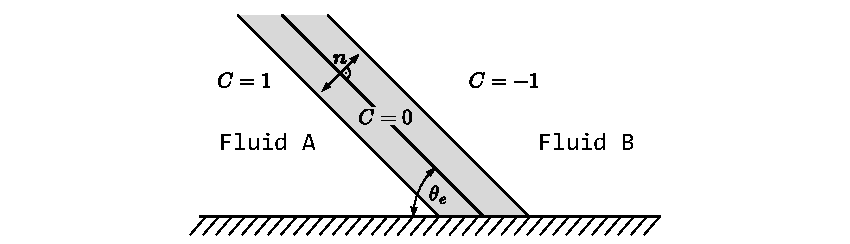
\includegraphics[width=.95\textwidth]{Pictures/DiffusiveInterface.pdf}
    \caption{Schematische Darstellung eines Diffusiven Interfaces}
    \label{fig: DiffusiveInteraface}
\end{figure}
In Abbildung \ref{fig: DiffusiveInteraface} ist die Kontakilinie eines Diffusiven interfaces dargestellt. Der Graue bereich ist der transitionsbereich des Ordnungsparameters und damit der Stoffgrößen. Innerhalb dieses Bereichs koexistieren beide Fluide mit ihren jeweiligen Dichten und viskositäten. Im Gleichgewichtszustand kann das Profil von $C$ normal zum Interface ermittelt werden, in dem die freie Energie (Gleichung \ref{eq: chempotentialMIXING_pahseFieldMethod})minimiert wird \cite{cai2015NumericalSimulationWetting}. Dies führt dann zu einer Beschreibung des Ordnungsparameters normal zum Interface mit
\begin{equation}
    \label{eq: InterfactialNormalDirProfile}
    C(n) = \tanh\left(\frac{n}{\sqrt{2}\epsilon}\right).
\end{equation}
Darin ist $n$ die normale auf dem Interface. Im gleichgewicht bleibt die Dicke des diffusen Interfaces gleich in einem Bereich von $3/\sqrt{2}\epsilon$ gilt für den Ordnungsparameter $-0.9\leq C\leq0.9$. Ebenfalls im Falle des Gleichgewichts, gleicht die Oberflächenspannung dem integral der freien energiedichte am Interface, woraus eine Beschreibung für die Oberflächenspannung abgeleitet werden kann \cite{jacqmin2000ContactlineDynamicsDiffuse}. 
\begin{equation}
\label{eq: surfacetensionEqui}
    \sigma = \int_{-\infty}^{\infty}\lambda\left( \frac{dC}{dn}  \right)^{2}= \frac{2\sqrt{2}}{3} \frac{\lambda}{\epsilon}
\end{equation}





\subsection{Wall Energy}






Jaqcmin \cite{jacqmin1999CalculationTwoPhaseNavier} postulierte eine Wandenergie der Form
\begin{equation}
    F_{\mathrm{w}}=\int \sigma g(C)dA, 
\end{equation}
womit die Wandenergie nur noch eine Funktion abhängig von der Fluidzusammensetzung direkt an der Wand abhängig ist. Die resultierende natürliche Phasenfeld Randbedingung mit lokalem thermischen Gleichgewicht ist gegeben mit
\begin{equation}
    \label{eq: BCfWall}
    \lambda \frac{\partial C}{\partial n_{\partial \Omega}} + f'_{\mathrm{w}}(C) =0.
\end{equation}
Mit $n_{\partial \Omega}$ als normalenrichtung auf der Wand (vgl. \ref{fig: DiffusiveInteraface}).
Die normalenrichtung zum interface kann mit der wandnormale und wand tangentiale Richtung auf der Wand beschrieben werden. 
\begin{equation}
    \label{eq: InterfaceNormal}
    n=n_{\partial\Omega}\cos{(\theta_{\mathrm{e}})}+\tau_{\partial\Omega}\sin{(\theta_{\mathrm{e}})}.
\end{equation}
Anschließend kann für den ersten Term aus Gleichung \ref{eq: BCfWall} mit den Gleichungen \ref{eq: InterfaceNormal}, \ref{eq: InterfactialNormalDirProfile} und \ref{eq: surfacetensionEqui} wie folgt erstellt werden
\begin{equation}
    \lambda\frac{\partial C}{\partial n_{\partial\Omega}} =\underbrace{\frac{3}{4}\sigma\left(1-C^2\right)\cos\theta_{\mathrm{e}}}_{=:-f'_\mathrm{w}(C)}.
\end{equation}
Daraus lässt sich eine Funktion für die Wandenergiedichte nach Integration ableiten\cite{jacqmin2000ContactlineDynamicsDiffuse}\cite{holzinger2021DirectNumericalSimulation}.
\begin{equation}
    f_{\mathrm{w}}(C)=-\sigma \cos\theta_e \frac{C(3-C^2)}{4} + \frac{\sigma_{S_L}+ \sigma_{S_V}}{2}
\end{equation}
Ist nur eine der Phasen anwesend, gibt diese Gleichung auch nur die jeweilige Oberflächenspannung zurück. Yue et al. \cite{yue2011WallEnergyRelaxation} weißt jedoch darauf hin, dass diese Beschreibung der Wandenergie für Gleichgewichtskontaktwinkel nahe $0^{\circ}$ oder $180^{\circ}$ nur schwer zu reproduzieren ist und das Modell nicht in der Lage ist precursor films zu handhaben. 



\section{Cahn-Hillard Navier Stokes Equations}
Die gekoppelten Cahn-Hillard Navier Stokes Gleichungen sind gegeben mit
\begin{align}
    \partial_t C + \nabla \cdot \left( C \mathbf{u} \right) &= -\nabla \cdot \mathbf{J} \\
    \nabla \cdot \mathbf{u} &= 0 \\
    \label{eq: NSEChanged}
    \partial_t(\rho \mathbf{u}) + \nabla \cdot (\rho \mathbf{u}\mathbf{u})&= -\nabla \tilde{p} + \nabla \mathbf{\tau} - \nabla \cdot(\mathbf{u}\mathbf{J})-\phi\nabla C + \mathbf{f}_{\mathrm{b}}
\end{align}

Darin ist $\tilde{p}$ ein modifizierter Druck, der aus dem Korteweg tensor entsteht, um die Kapillarität zu berücksichtigen. Die Annahme eines Newtonschen Fluids gilt $\mathbf{\tau} = 2\mu \mathrm{dev}\mathbf{D}$ mit $\mathbf{D} = 1/2[\nabla \mathbf{u}+(\nabla \mathbf{u})^{\mathrm{T}}]$ als Deformationstensor. Weiter ist die Dichte $\rho$ und viskosität $\mu$ volumetrisch gemittelt mit 
\begin{equation}
    \rho = \frac{1 + C}{2} \rho_1 +\frac{1 + C}{2} \rho_2.
\end{equation} 
Darin sind die suffixe $1$ und $2$ Markierungen für die jeweiligen Phasen. Die Viskosität wird analog berechnet. Der Term $- \nabla \cdot(\mathbf{u}\mathbf{J})$ ist notwendig, um die thermische consistenz zu gewährleisten \cite{ding2007DiffuseInterfaceModel}. $\mathbf{J}$ ist der phase-field flux und nach Landau und Lifshitz \todo{cite} gilt $\mathbf{J} = -M\nabla \phi$ 

\chapter{Case Setup}
\label{chap: CaseSetup}
Die Geometrie und einige Stoffeigenschaften sind durch die in \ref{chap: wettingTheory} definierten vereinfachungen und Annahmen bereits vorgegeben. Im folgen wird zu beginn die Geometrie der Kapillare vorgestellt, gefolgt von den Materialeigenschaften und verwendeter Randbedingunen. Da mehrere Untersuchungen unternommen wurden, erfolgt in Kapitel eine Übersicht über die durchgeführten Simulationen und dessen Initialiserung. 


Wie bereits in Kapitel \ref{chap: Introduction} geschrieben, erfolgen die Simulationen mit dem solver \texttt{phaseFieldFoam}. Dieser wurde bereits mehrfach Validiert, worauf in Kapitel \ref{chap: Validation} genauer eingegangen wird.
\section{Geometry}
Die Geometrie der Kapillare wird so angenommen, dass sie wie in Abbildung \ref{fig: Capillary Geometry} zu sehen ein Reservoir mit Wasser hat, welches durch Oberflächeneffekte in die Kapillare strömt. Durch die Annahme, dass sich ein Teil des Wassers bereits in der Kapillare befindet, wird in der Simulieren Geometrie lediglich die Randbedingung so gesetzt, dass das Wasser in diesem Reservoir nachströmen kann. Die Dimensionen der Kapillare ergeben sich daraus, dass die Simulation der Kapillare perspektivisch auch mit experimenten verglichen werden soll. Daher wurden auch weitere, komplexere Geometrien simuliert, die jedoch nciht Teil dieser Arbeit sind. 
Wie zu erkennen, handelt es sich um eine Kapillare mit lediglich $6nm$ Durchmesser. Eine Simulation so kleiner Kapillare wurde soweit bekannt bisher nicht mit der Phasenfeld methode Simuliert.

\begin{figure}[h]
    \centering
    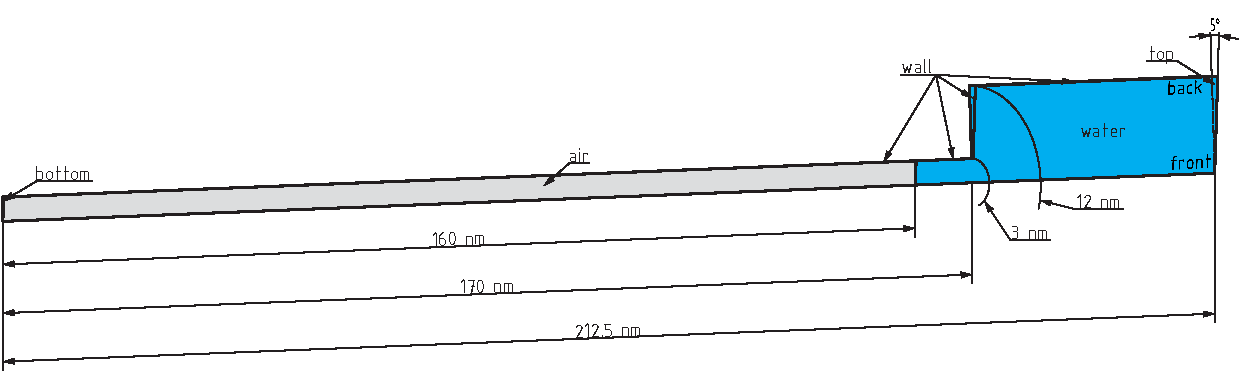
\includegraphics[width=.95\textwidth]{Pictures/Cap_5DEG.pdf}
    \caption{Schematic of used Capillary}
    \label{fig: Capillary Geometry}
\end{figure}

Die Diskretisierung der Geometrie wurde so gewählt, dass die Elemente eine Kantenlänge von $0.2nm$ haben. In Radialer Richtung hat eine Wedge nur ein Element. Zur erstellung der \texttt{blockMeshDict}-datei, wurde ein python skript erstellt, welches anhand des Kapillardurchmessers und länge eine Datei mit den in Abbildung \ref{fig: Capillary Geometry} dargestellten Benennungen der Oberflächen erstellt. 

\section{Randbedingunen}
In Abbildung \ref{fig: Capillary Geometry} sind neben der Geometrie auch die Flächen, die mit Randbedingungen versehen wurden benannt. Die Flächen \texttt{front} und \texttt{back} sind sich gegenüberliegende Flächen der Wedge und müssen dementsprechende Ranbedinungen erhalten. Die \texttt{wall} Flächen sind nicht durchdringbare Oberflächen und \texttt{top}, bzw. \texttt{bottom} Oberflächen durch die ein Fluss zugelassen wird.
Die wesentlichen Randbedingunen an der Wand sind in Tabelle \ref{tab: BoundaryConditions_wall} aufgelistet. 

\begin{table}[h]
    \centering
        \caption{relevant boundary conditions wall}
        \label{tab: BoundaryConditions_wall}
        \begin{tabular}{lll}
            Parameter & Value \\ \hline
            orderparameter $C$ & \texttt{equilibriumPhaseContactAngle}     \\
            equilibrium contact angle $\theta_{\mathrm{e}}$ & $15^{\circ}$, $45^{\circ}$, $75^{\circ}$\\
            chemisches Potential $\phi$   & \texttt{zeroGradient}        \\ 
            velocity $\mathbf{u}$ &   $\mathbf{u_{\mathrm{w}}} = 0$\\
            pressure $p$&  \texttt{fixedFluxPressure} \\
        \end{tabular}
\end{table}
Für den Ordnungsparameter $C$ wird die Gleichgewichtsrandbedingung angenommen und der Gleichgewichtskontaktwinkel für jede der drei Simulationen mit dieser Geometrie mit $15^{\circ}$, $45^{\circ}$ bzw. $75^{\circ}$ angegeben. Der Gradient des chemischen potentials an der Wand wird als null gesetzt, genauso wie die Geschwindigkeit der Wand. Die Ranbedingung für den Druck wird mit \texttt{fixedFluxPressure} so gewählt, dass der Druckgradient so angepasst wird, das der Massenfluss am Rand mit der vorgegebenen Geschwindigkeit an der Wand übereinstimmt. 

\section{Materialeigenschaften}
Für die Simulation werden unter anderem Wasser und Luft bei $25^{\circ}$ Celsius als Medium angenommen. Damit folgen die in Tabelle \ref{tab:physicalProperties_CaseSetup} dargestellten Materialeigenschaften. 
\begin{table}[h]
    \centering
    \caption{Physical properties}
    \label{tab:physicalProperties_CaseSetup}
    \begin{tabular}{lll}
    fluid & density ($\frac{kg}{m^3}$) & kinematic viscosity $\frac{m^2}{s}$ \\ \hline
    water & $1000$                     & $1.00E-06$                          \\
    air   & $1$                        & $1.00E-05$                          \\ 
    \end{tabular}
    \end{table}


\section{Simulationsparameter}




\section{Auswertungsmethoden}
Zur Auswertung der Simulation wurde unter anderem die Anwendung \texttt{paraview} verwendet. Alle bilder der Simulation wurden damit erzeugt. Die Auswertung und darstellung abgeleiteter oder berechneter Größen in Diagrammen wurden hingegen mit der python bibliothek \texttt{Matplotlib} erzeugt. Dazu wurde ein skript erstellt, das die Ergebnisse der function obsjects sammelt und gegebenenfalls Berechnungen damit vornimmt. 
\paragraph{function objects}
Mit hilfe von function objects können während der laufenden Simulation daten erfasst werden. \texttt{phaseFieldFoam} liefert einige funktionen zum auslesen der Simulation mit, die auch hier verwendet werden. Diese Müssen in der \texttt{controlDict} datei eingebunden und konfiguriert werden. 


\chapter{Validation}
\label{chap: Validation}
The \texttt{phaseFieldFoam}- Solver 


src \todo{bodziony2023, Cai2015, woerner2021, Samkhaniani2021, holtzinger, marianna?, hagg?(sogar mit wedge und amr)}

\chapter{Results}
\label{chap: Results}
Im Folgenden werden die Resultate der durchgeführten Simulationen analysiert. Ziel ist es, eine Erklärung für den Übergang zwischen den vorgestellten Wachstumsregionen des kapillaren Aufstiegs zu finden. Insbesondere wird der Übergang vom linearen Bereich ($z(t)\sim t$) zum von Lucas und Washburn beschriebenen Wachstum ($z(t)\sim \sqrt{t}$) betrachtet. Um potenzielle Einflüsse durch verschiedene Kontaktwinkel zu berücksichtigen, wurden die Simulationen mit drei unterschiedlichen Werten durchgeführt. Zusätzlich wurden Simulationen mit aktivierten Ungleichgewichtsrandbedingungen durchgeführt, um den Einfluss einer Relaxation an der Wand auf den kapillaren Aufstieg zu analysieren. 
Zunächst wird die Gleichgewichtsrandbedingung in Kapitel \ref{sec: EquilibriumBoundaryCondition} untersucht, gefolgt von einem Vergleich mit der Ungleichgewichtsrandbedingung im Abschnitt \ref{sec: outOfEquilibriumBoundaryCondition}. 

Wie in Kapitel \ref{chap: CaseSetup} beschrieben, hat die Gravitation keinen Einfluss auf die durchgeführten Simulationen gehabt. Damit wird jedoch auch klar, dass eine der besprochenen von Lucas und Washburn angenommen Vereinfachnungen für diesen Fall nicht gilt und eine Abweichung der vorhersage gemäß Gleichung \ref{eq: LW-Eq} darauf zurückzuführen ist, dass ein Gleichgewicht zwischen Kapillarkraft und viskosem drag nicht ausreicht, um den Kapillaren Aufstieg in frühen imbibitionsstadien zu beschreiben.


\section{Equilibrium Boundary Condition} 
\label{sec: EquilibriumBoundaryCondition}
Die auswertung mit nur einem der verwendeten Kontatkwinkel findet im folgenden mit einem Gleichgewichtskontaktwinkel von $\theta_{\mathrm{e}}=15^{\circ}$ statt. Ein Vergleich der Simulationsergebnisse für diesen Kontaktwinkel mit der Lucas-Washburn-Gleichung \ref{eq: LW-Eq} ist in Abbildung \ref{fig: LW-PFF_comp} dargestellt. Die vorhergesagte imbibitionslänge wird als linie in rot und die Ergebnisse der Simulation als Punkte in dunkel blau abgebildet. Um die gleiche Größenordnung wie die Simulation vorherzusagen, musste ein Korrekturfaktor zur Lucas-Washburn-Gleichung hinzugefügt werden, was allerdings nicht verwundert aufgrund der kleinen Geometrie und frühen Zeitpunkte (wie bereits in Kapitel \ref{chap: wettingTheory} gezeigt).
\begin{figure}[h]
    \centering
    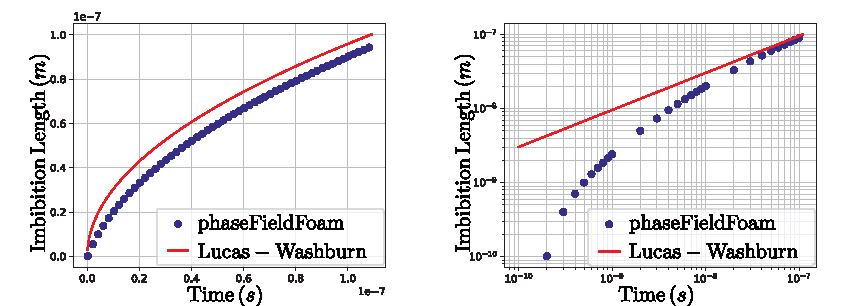
\includegraphics[width=.95\textwidth]{Pictures/LW-lin_loglog.pdf}
    \caption{Vergleich des von Lucas-Washburn vorhergesagten Wachstums mit den Ergenissen von \texttt{phaseFieldFoam}}
    \label{fig: LW-PFF_comp}
\end{figure}
In Abbildung \ref{fig: LW-PFF_comp} (a) erfolgt eine lineare und in \ref{fig: LW-PFF_comp} (b) eine logarithmische Skalierung der Daten. Es wurden zur besseren Übersicht nicht alle vorhanden Datenpunkte der Simulation geplottet, da diese vor allem in der logarithmischen Darstellung sich gegenseitig überlagern würden und die darstellung unübersichtlich machen würden. \todo{ggf anhang mit weiteren plots ohne n\_th??} 
In der linearen Darstellung wird bereits deutlich, dass das Aufstiegsverhalten sich vom vorhergesagten unterscheidet. In der logarithmischen Darstellung werden die Unterschiede noch deutlicher. Anfangs ist die Steigung der Simulationsergebnisse größer als die der Vorhersage, bis sie schließlich konvergieren. Dies deutet darauf hin, dass der kapillare Aufstieg erst nach einer gewissen Zeit dem bekannten Lucas-Washburn-Wachstum folgt, was auch von vielen in Abschnitt \ref{sec: capillaryRise} zitierten Arbeiten bestätigt wird. 

Um die Unterschiede im Verhalten zu verstehen, ist es sinnvoll, die in der Wassersäule wirkenden Kräfte zu betrachten. Delanoy et al. \cite{delannoy2019DualRoleViscosity} führten diese Unterschiede auf eine lokale Dissipation an der Kontaktlinie zurück. Daher ist es ratsam, den Bereich nahe der Schnittstelle genauer zu betrachten. In Abbildung \ref{fig: eDiss_wedge} werden die viskosen Kräfte in der Wassersäule nahe der Kontaktlinie dargestellt für einen Zeitpunkt von $100ns$ nach Beginn. Dieser Bereich wird fokussiert, da in anderen Teilen der Wassersäule die Kräfte deutlich geringer sind. Es ist deutlich zu erkennen, dass nahe der Kontaktlinie und direkt an der Wand die viskosen Kräfte am größten sind und sich zwei dissipative Kanäle ausbilden. Hier überlagern sich die viskosen Kräfte nahe der Kontaktlinie und der viskosie Widerstand, hervorgerufen durch die Veränderungen des Kontaktwinkels aufgrund der Dynamik des Systems. \todo{check!!!!}

\begin{figure}[h]
    \centering
    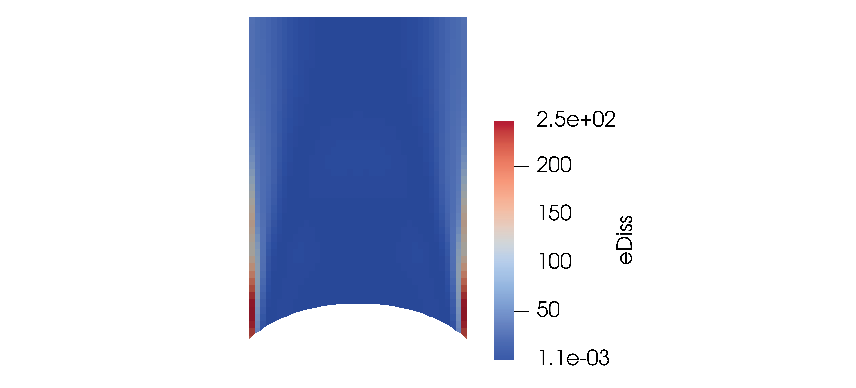
\includegraphics[width=.95\textwidth]{Pictures/eDiss_Wedge.pdf}
    \caption{Dissipative channels near the contact line.}
    \label{fig: eDiss_wedge}
\end{figure}

\begin{figure}[h] 
    \centering
    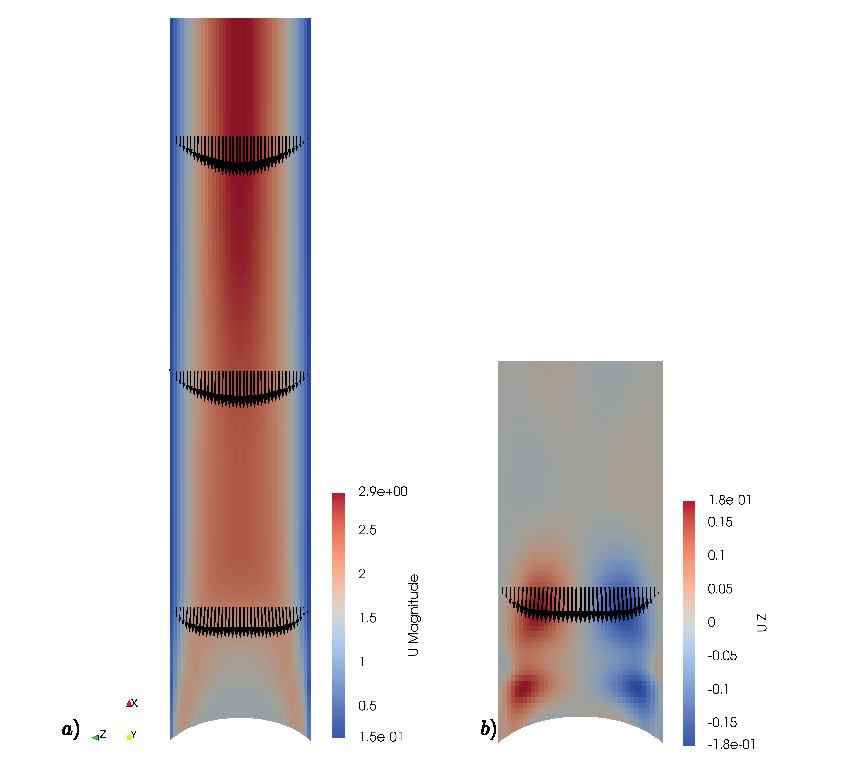
\includegraphics[width=.95\textwidth]{Pictures/Velo_Wedge.pdf}
    \caption{(a) Velocity field in the water column at $100ns$ and $\theta_{\mathrm{e}}=15^{\circ}$, (b) detailed view of recirculation near the interface.}
    \label{fig: Velofield_Wedge}
\end{figure}
In Abbildung \ref{fig: Velofield_Wedge} wird das Geschwindigkeitsfeld im Wasser visualisiert und entspricht den Erwartungen. In der Mitte der Kapillare ist die Geschwindigkeit des Wassers am höchsten (vgl. (a)). Zur Visualisierung des sich verändernden Geschwindigkeitsfeldes bei annäherung an das Interface wurden ebenfalls für drei Ebenen die Vektoren des Geschwindigkeitsfeldes hinzugefügt. Weit vom Interface entfernt, liegt das erwartete parabolische Profil vor. Bei näherung an das Interface ist deutlich zu erkennen wie die Strömung in der Mitte abgebremst wird und bei genauer betrachtung ist anhand der Vektoren auch zu erkennen, dass die Strömung an den Rand abgelenkt wird. Dazu wurde in (b) der Ausschnitt nahe des Interface vergrößert und statt der Magnitude der Geschwindigkeit nur die Komponente normal zur Strömungsrichtung ($z$-Richtung) visualisiert. Es ist deutlich zu erkennen, dass bis kurz vor der Strömung diese Komponente vernachlässigbar ist und nahe des Interface stark ansteigt und zwei Regionen zu bilden scheint. Eine direkt am Interface und nahe der Wand und ein weiteres etwas weiter innerhalb der Wassersäule. Anahnd der Legende ist deutlich erkennbar, dass die Größenordnung im Vergleich zur Geschwindigkeit in Strömungsrichtung sich um eine Dekade unterscheidet. Der Bereich in dem die Änderung der Geschwindigkeit stattfindet, wird im folgenden als $\mathrm{W}$ bezeichent. Bis zu diesem Bereich kann angenommen werden, dass die Strömung der von poiseuille beschriebenen entspricht und damit der Viskose Widerstand dem Poseuille viskosen Widerstand entspricht. Damit können dann die in $\mathrm{W}$ herrschenden viskosen Kräfte direkt aus der Simulation berechnet werden. 



Die insgesamt wirkenden viskosen Kräfte erhält man aus der Simulation mit Gleichung \ref{eq: totalViscForce} und der viskosen Wiederstand kann mit $F_{\eta}$ aus Gleichung \ref{eq: NewtonBalanceForcesOnly} berechnet werden. Die Differenz der beiden Kräfte entspricht dann den in $\mathrm{W}$ herrschenden viskosen Kräften. 
Die Geschwindigkeit zur Berechnung des viskosen Widerstandes wurde über die Position des Meniskus und den jeweiligen Zeitschritt berechnet. Zum weiteren Vergleich wurden die erwarteten viskosen Kräfte nicht nur über die beschriebene Differenz, sondern auch aus der von Ruiz et al. \cite{ruiz-gutierrez2022LongCrossoverDynamics} abgeleiteten Gleichung \ref*{eq: meniscusFormation}. Diese Berücksichtigt den dynamischen Kontaktwinkel, welcher über die Cox-Voinov Gleichung \ref*{eq: Cox-Voinov}, ebenfalls mit der Geschwindigkeit berechnet wurde. Für das Verhältnis der Längenskalen wurde die Länge der Kapillare auf eine cutoff length von $1 nm$ bezogen.
%Da eine Automatische auswertung der Position des Beginns von $\mathrm{W}$ nicht umsetzbar war, wurde händisch anhand einiger Stichproblem die größe für unterschiedliche Zeitpunkte und Kontaktwinkel bestimmt. Die größe des Bereichs schwankte dabei immer um $\approx 6-8nm$. \todo[inline]{CHEKCEN BEI ANDEREN WINKELN!!! und ob es drin bleibt!!!}\todo{entspricht eher den Kräften ohne poseuille, oder?}
%Darüber hinaus wird mittels der Geschwindigkeit des Meniskus auch der theoretische, Poiseuille viskose Widerstand und die Widerstandkräfte am Meniskus (Gleichung \todo{EQ}) berechnet. Hierbei wird die von Cox und Voinov beschriebene Gleichung (\ref*{eq: Cox-Voinov}) zur Vorhersage des dynamischen Kontaktwinkels verwendet. Das Verhältnis der Längenskalen ist meist schwer abzuschätzen, da für $l_{\mathrm{m}}$ meist eine Länge von $1nm$ angenommen wird und für $l$ mehrere Lägen, wie der Radius, die Länge der Kapillare oder auch die Länge von $\mathrm{W}$ wird im folgenden ein Verhältnis von $l_{\mathrm{m}}/l\approx10$ angenommen. 
\todo{Woher kommt das?}
\todo{Bild oder beschrieben der rezikulation} 

\begin{figure}[h]
    \centering
    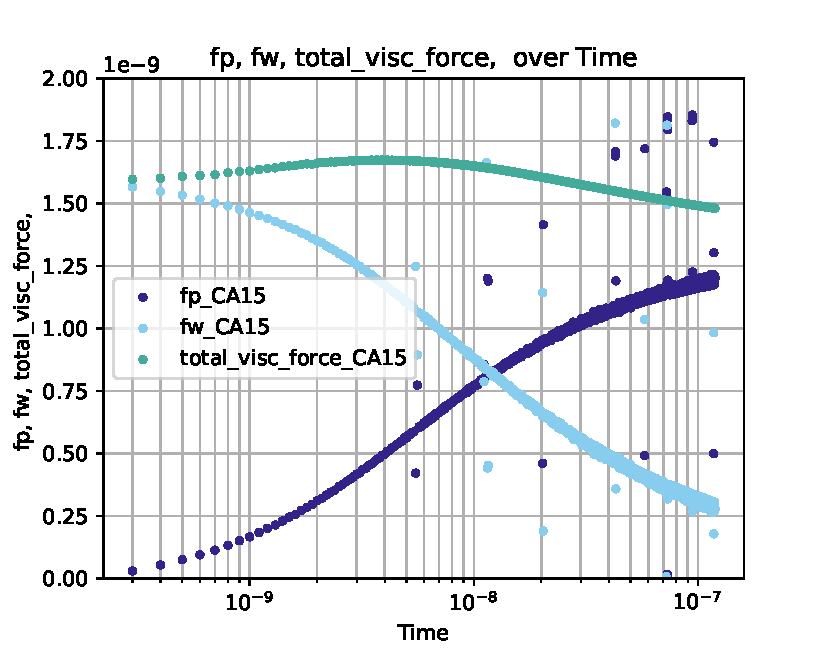
\includegraphics[width=.95\textwidth]{Pictures/loglog_fp_fw_total_visc_force_overTime.pdf}
    \caption{Viscous forces over time}
    \label{fig: forcesOverTime}
\end{figure}

Plottet man diese Kräfte (siehe  Abbildung \ref*{fig: forcesOverTime}) in einem Diagramm wird deutlich, wie zu Beginn der imbibition die Kräfte aus der Meniskusbildung die viskosen Kräfte überwiegen und erst nach einiger Zeit die viskosen Kräfte übernehmen und anschließend dominieren. Delanoy hat postuliert, dass ab einer imbibitionslänge von $z \sim r\cdot ln(r/l_s)$ die viskosen Kräfte überwiegen. Das würde bedeuten bis zu einer imbibition von $\approx 3.3nm$ überwiegen nach Delanoy die Poiseuille Reibung vernachlässigbar ist. Ein Vergleich mit Abbildung \ref*{fig: LW-PFF_comp} zeigt, dass der Meniskus diese nach $\approx 1ns$ zurückgelegt hat. Zu diesem Zeitpunkt ist der Anteil der Poseuille viskosen Kräften bei $\approx 14\%$. Unmittelbar danach nehmen diese deutlich zu und gleichen schließlich nach $\approx 10ns$ den Anteil der Meniskus Kräfte aus. Der Vergleich mit Abbildung \ref*{fig: forcesOverTime} b) zeigt, in diesem Bereich ($\approx 1ns$) der Übergang von $t\sim t$ zu $t\sim \sqrt{t}$ beginnt und schließlich bei $\approx 10ns$ bereits nahezu abgeschlossen ist.



Im Abschnitt \ref{sec: CA_Measurement} wurden zwei Methoden vorgesetellt, die verwendet werden können, um den Kontaktwinkel der Simulation zu Messen. Da aufgrund der Theoretisch berechneten Kontaktwinkel über die Cox-Voinov Gleichung \ref*{eq: Cox-Voinov} für den Winkel andere Ergebnisse e

Zur Berechnung des Kontaktwinkels können die in Abschnitt \ref*{sec: CA_Measurement} vorgestellten Methoden verwendet werden. Wie in Kapitel \ref*{chap: wettingTheory} beschrieben wird davon ausgegangen, dass sich der Meniskus zu einem Kreissegment entwickelt. Da in diesem Fall nur der Kontaktwinkel benötigt wird, kann auf eine in \cite{buttPhysicsChemistryInterfaces} vorgestellte Gleichung zurückgegriffen werden, womit sich der Kontaktwinkel mit 

berechnen lässt. Die variablen und wie sie erhalten werden ist bereits in Kapitel \ref*{chap: Validation} beschrieben. \todo{add cox angles to compare in one plot and just 15deg case}
\begin{figure}[h]
    \centering
    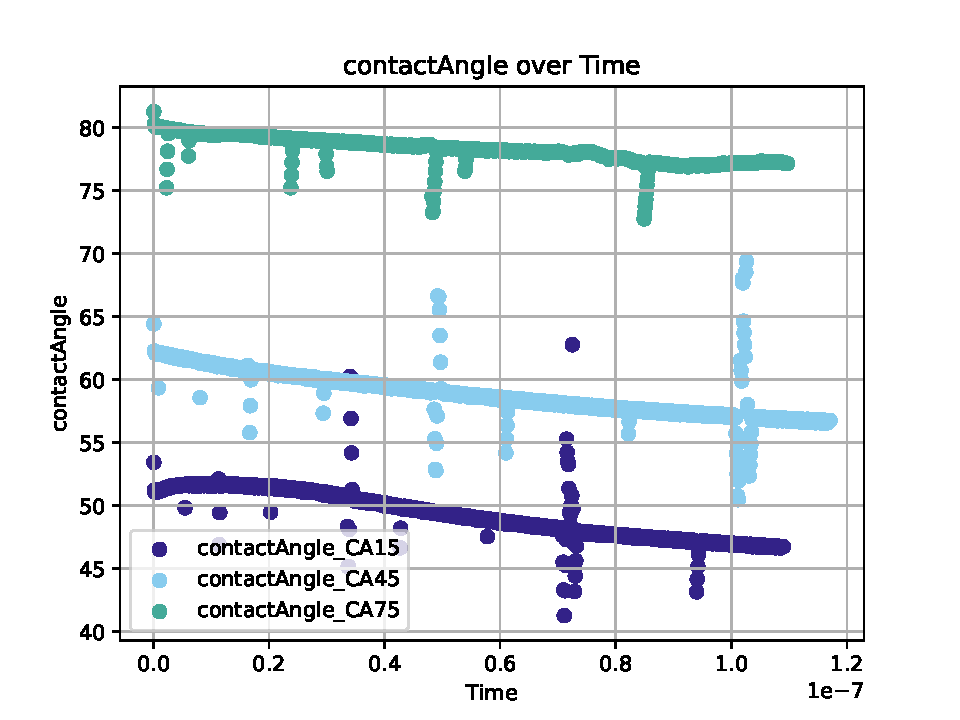
\includegraphics[width=.95\textwidth]{Pictures/contactAngle_overTime.pdf}
    \caption{computed contact angle over time }
    \label{fig: CA_overTime}
\end{figure}
Darin ist zu sehen, dass sich sehr schnell ein Winkel einstellt,... \todo{ausformulieren mit Daten vom feineren Netz.}


%Diese erkenntnis bestätigt sich, wenn man die Steigung der SImulaiton an einigen Stichproben ermittelt. Dabei wird deutlich, dass die Steigung asymptotisch %auf den Wert der Lucas-Washburn Gleichung zustrebt. \todo{add table with slope values for some probes}




\subsection{Contact Angle Variation}
Wie zuvor erwähnt wurden die Simulationen für mehrere Kontaktwinkel durchgeführt, um mögliche Einflüsse bewerten zu können. Es ist zu erwarten, dass der Kontaktwinkel einen einfluss auf die Geschwindigkeit hat, mit der die Wassersäule aufsteigt, was sich auch in den Daten wiederspiegelt (vgl. Abbildung \ref{fig: CAVar_z_overTime}). 
\begin{figure}[h]
    \centering
    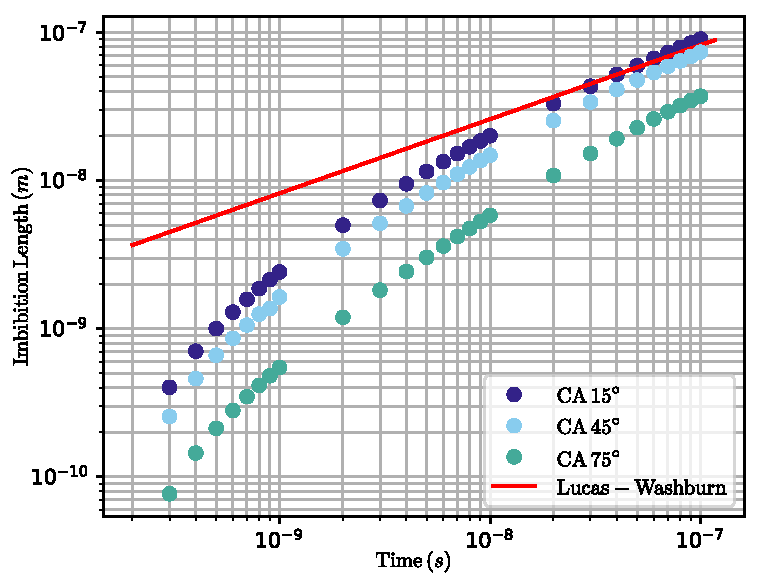
\includegraphics[width=.95\textwidth]{Pictures/loglog_z_over__time_CA_Var.pdf}
    \caption{Imbibition height over time for different contact angles in logarthmic presentation.}
    \label{fig: CAVar_z_overTime} 
\end{figure}
In Abbildung \ref{fig: CAVar_z_overTime} wurde wie zuvor die imbibitionslänge über die Zeit in logarithmischer Darstellung visualisiert. Die rote Linie ist auch hier wieder eine angepasste Version der Lucas Washburn Gleichung für den Gleichgewichtskontaktiwnkel $\theta_{\mathrm{e}}= 15^{\circ}$. Für jede der Simulationen ist das gleiche verhalten zu beobachten. Zu Beginn ist die Steigung größer und nähert sich mit fortlaufender Zeit an $z(t)\sim \sqrt{t}$ an. Auch hier wurden zur besseren Darstellung Punkte nicht dargestellt, die nicht zum logarithmus passen. Diese Ergebnisse entsprechen der Erwartung, dass mit höherem Kontaktwinkel die Geschwindigkeit des Aufstiegs abnimmt.

Interessanter ist ein Vergleich der Kräfte, genauer eine Betrachtung der Anteile der Kräfte in Abbildung \ref{fig: CA_Forces}. Bildet man wie zuvor die Viskosen Widerstandskräfte und bezieht diese auf die ingesamt wirkenden viskosen Kräfte, kann auf das vorliegende Wachstumsverhalten geschlossen werden. Liegt dieses Verhältnis näher bei $1$, folgt der Kapillare aufstieg den Lucas-Washburn Gesetzmäßigkeiten, für Werte nahe $0$, einem linearen Wachstum. Die darstellung über die Zeit zeigt, dass mit verändertem Gleichgewichtskontaktwinkel die Zeit beeinflusst wird, bis die viskosen Kräfte überwiegen. Ändert man die Darstellung so, dass das Kräfteverhältnis über die imbibitionslänge aufgetragen wird, wird deutlich, dass der Kontatkwinkel in dieser Betrachtung keine Rolle zu spielen scheint. 

\begin{figure}[h]
    \centering
    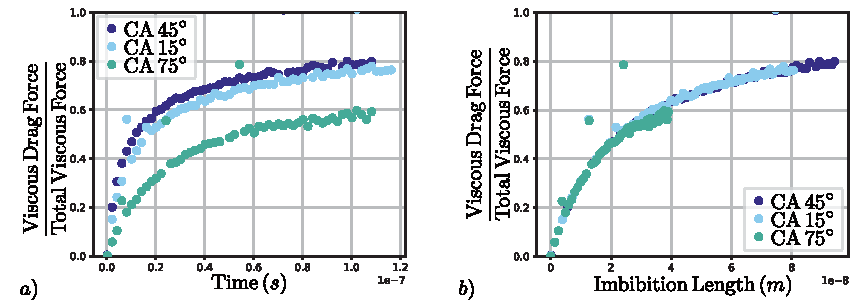
\includegraphics[width=.8\textwidth]{Pictures/CA_Forces_Variation.pdf}
    \caption{computed contact angle over time }
    \label{fig: CA_Forces} 
\end{figure}
Da wie erwartet die Simulation mit einem Kontaktwinkel von $\theta_{\mathrm{e}}=75^{\circ}$ die langsamste ist, liegen hier keine genauen Erkenntnisse vor wie sich das Verhältnis weiterentwickelt. Es ist jedoch zu Erahnen, dass hier eine Änderung des Verhaltens beginnt. Die Vermutung liegt nahe, dass die Simulation im Begriff ist den Gleichgewichtszustand zu erreichen und damit auch der Viskose Widerstand nicht mehr weiter ansteigt. Diese Vermutung wird durch eine Darstellung der Kontatktwinkel untermauert. \todo{add image and chapter where the different methods are explained!}




\section{out of equilibrium boundary condition}
\label{sec: outOfEquilibriumBoundaryCondition}
Zu Beginn ein Hinweis zu den Simulationen mit dieser Randbedingung. Leider ist es aufgrund der schelchten Sichtbarkeit in der aktuellsten Version von \texttt{paraview(5.11.1)} nicht möglich so kleine geometrien als oberflächenmodell darzustellen. Daher war nur eine Visualisierung des Gitters möglich, was jedoch, wie sich später gezeigt aht, probleme der Simulation maskiert hat. Erst zu einem späteren Zeitpunkt wurde auf eine ältere Version (\texttt{paraview(5.8.1)}) gewechselt. In dieser ist die visualisierung ohne Problem möglich und die Probleme der Simulation wurden sichtbar. Bei dem Problem handelt es sich um Drücke in Wand und Interface nähe, die mit dauer der Simulation größer zu werden scheinen. Ob es sich dabei wirklich um ein Problem oder möglicherweise nicht handelt konnte leider aufgrund fehlender Zeit nicht mehr untersucht werden. 

Da das aufstiegsverhatlen der Simulationen dennoch physikalisch erscheint, werden die Ergenisse dennoch vorgestellt und untersucht. Es bleibt jedoch festzuhalten, dass diese Ergebnisse mit vorsicht zu genießen sind und in jedem Fall weiterer tests bedürfen vor allem, weil sie mit fortlaufender Zeit in nähe des Interfaces auftreten und dieses auch beeinflussen zu scheinen. 
\todo{Simulationen laufen. ggf. erwähnen und anmerken, ob und wenn ja wie, sich diese auswirken oder geändert haben. }

Bisher wurden alle auswertungen der Simulationen ohne die annahme einer Diffusion an der Wand und damit der annahme einer ideal Glatten Wand. In Abbildung \ref{fig: HDT_MKT_comp} (c) wurde eine molekulare wand illustriert. Trotz der angedeuteten unebenheiten würde diese wand vermutlich bereits einer ideal glatten wand gleichen. Allein aufgrund der tatsache, dass atome rund sind, kann keine ideal glatte ebene existieren. Eine simulation auf atomarer Ebene ist mit großem aufwand verbunden und um effekte der Wand dennoch abbilden zu können wurde in abschnitt \ref{sec: nonEquiBC} die Ungleichgewichtsrandbedingung eingeführt. Mit dem vorgestellten Faktor kann die Rauigkeit der Wand modelliert werden, desto größer der Wert, desto geringer die modellierte Dissipation an der Wand. 



\chapter{Outlook}
\label{chap: Outlook}
\begin{itemize}
    \item complex geometry
    \item temperature dependent capillary rise?
    \item surfactants and capillary rise?
    \item more fluids with other viscosisties
    \begin{itemize}
        \item as delanoy discussed the viscosity plays a major role in the capillary rise
    \end{itemize}
    \item in depth reseach of gamma value and possible dependence of mesh resolution
\end{itemize}



\section{Complex Geometry}
In experiments it is not possible to generate a capillary with a constant diameter. Therefore a geometry with a more realistic geometry is also simulated. To create the porous medium for the experiments, "spheres" are used in a pour. The area between the spheres of this fill is then filled and the spheres are dissolved. This creates capillaries that are not ideally smooth as previously assumed, but rather a shape like in figure (\todo[inline]{ref to a picture with used geometry}). It was assumed in a simplified way that no bridges are created between capillaries in this process. Furthermore, it is assumed that the spheres are ideally aligned with each other at the beginning of the process.  \todo{Check, if correct!} 
In this case it is assumed, that the centre of the circle is in the middle of a segment and only displaced by an offset from the x-axis. The connection between the segments is to make sure the mesh is sufficient. 

The numerical setting keep the same as in the wedge case with a cylindrical capillary. 


To simulate the imbibition process we use the \verb|OpenFoam| framework. To get a estimation of the necessary parameters, a previously validated case is reused and adapted to this case. First the simulation is assumed to be axissymmetric. Therefore a Wedge is used for the major part of the simulations. To validate the results of the wedge a 3D simulation was performed, too. 

The necessary geometry, settings and boundary conditions for each case are described below. 


\printbibliography

\end{document} 
